%% FL-Iroh -- Elsevier CAS (cas-dc) double-column manuscript
%% Ported from paper.tex (IEEEtran). English only.
%% Compile from this directory so the cas-dc.cls / cas-common.sty are found.

\documentclass[a4paper,fleqn]{cas-dc}

% cas-dc already loads: graphicx, amsmath/amsfonts/amssymb, booktabs,
% makecell, multirow, array, colortbl, dcolumn, xcolor(svgnames,dvipsnames),
% hyperref(colorlinks), fontenc(T1). Do NOT reload those.

\usepackage[utf8]{inputenc}
\usepackage[numbers]{natbib}   % numeric [n] citations, matches thebibliography
\usepackage{tikz}
\usetikzlibrary{arrows.meta, positioning, shapes.geometric, calc}
\usepackage{pgfplots}
\pgfplotsset{compat=1.18}

% Absorb minor overfull \hbox boxes in the narrow two-column measure
\emergencystretch=3em
\tolerance=800

\begin{document}
\let\WriteBookmarks\relax
\def\floatpagepagefraction{1}
\def\textpagefraction{.001}

\shorttitle{FL-Iroh: NAT-Transparent Federated Learning for Agricultural and Environmental IoT}
\shortauthors{R.~L\'{o}pez-Blanco et~al.}

\title[mode = title]{FL-Iroh: NAT-Transparent Federated Learning for Agricultural and Environmental IoT via QUIC P2P Transport and CoAP Service Discovery}

% ---- Authors --------------------------------------------------------------
\author[1]{Ra\'{u}l L\'{o}pez-Blanco}[orcid=0000-0002-8856-4008]
\cormark[1]
\ead{raullb@usal.es}

\affiliation[1]{organization={BISITE Research Group, University of Salamanca},
            addressline={Edificio I+D+i, Calle del Espejo 2},
            city={Salamanca},
            postcode={37006},
            state={Castille and Leon},
            country={Spain}}

\author[2,3]{Ricardo S.~Alonso}[orcid=0000-0002-6599-0186]
\ead{ralonso@air-institute.com}

\affiliation[2]{organization={AIR Institute -- Deep tech lab, IoT Digital Innovation Hub},
            addressline={Paseo de Bel\'{e}n 9A},
            city={Valladolid},
            postcode={47011},
            state={Castille and Leon},
            country={Spain}}

\author[1]{Javier Prieto}[orcid=0000-0001-8175-2201]
\ead{javierp@usal.es}

\author[3]{Tiago Pinto}[orcid=0000-0001-8248-080X]

\affiliation[3]{organization={University of Tr\'{a}s-os-Montes and Alto Douro},
            city={Vila Real},
            country={Portugal}}

\cortext[1]{Corresponding author}

% ---- Abstract -------------------------------------------------------------
\begin{abstract}
Federated Learning (FL) for agricultural and environmental IoT faces a practical connectivity barrier: edge devices deployed behind Network Address Translators (NAT) and Carrier-Grade NAT (CGNAT) cannot host or expose an aggregation endpoint without static IP allocations, VPN overlays, or third-party cloud relays. We present FL-Iroh, an open-source FL system that embeds NAT traversal in the transport layer itself, coupling the Iroh QUIC-based peer-to-peer transport with a CoAP/CoRE control plane for service discovery and round coordination. Peers are addressed by public key rather than by IP address, and an end-to-end-encrypted relay guarantees connectivity whenever a direct path cannot be formed. In real-hardware tests between a PC and a Raspberry Pi~4B on different ISPs 300~km apart, every session connected, and 118 of 120 WAN transfers (98.3\%) used a direct QUIC hole-punched path---including under CGNAT, symmetric NAT, and a port-443-only firewall---with the relay never exercised; a repeated cold-start campaign further established a direct path on 145 of 150 independent connection attempts (96.7\%, 0\% relay). The transport is algorithm-agnostic: the same QUIC channel federates a compact neural network for crop recommendation (AgriMLP, 7.7K parameters) and, for seven-day-ahead air-quality forecasting across ten Castilla y Le\'on monitoring zones, both a neural baseline and a federated Prophet GAM under two aggregation rules (FedAvg and the partial-aggregation FedGAM). The Prophet model reaches 57.9\% test accuracy against a 47.5\% seven-day persistence baseline, while a same-model ablation shows the aggregation rule itself is not the driver ($\Delta{<}0.3$pp, $p{=}0.35$). FL-Iroh shows that FL can be deployed across NAT-constrained agricultural and environmental IoT without static IPs, VPN overlays, or per-node system daemons.
\end{abstract}

\begin{highlights}
\item NAT traversal embedded in the FL transport: peers addressed by public key, no routable server IP, VPN, or per-node daemon required.
\item Direct QUIC hole-punching carried 98.3\% of WAN transfers (118/120) under NAT, CGNAT and port-443 firewall scenarios; every session connected, with an end-to-end-encrypted relay as guaranteed fallback.
\item Lightweight CoAP/CBOR control plane for round coordination and discovery; millisecond-scale round signaling, with capability-based semantic filtering scaling linearly in network size.
\item Algorithm-agnostic transport federates both neural networks and statistical GAMs (Prophet/FedGAM) with a single server-side change, validated by a same-model aggregation ablation.
\item Evaluated on agricultural (crop recommendation) and environmental (Castilla y Le\'on air quality) tasks on real PC$\leftrightarrow$Raspberry~Pi hardware across a 300~km WAN.
\end{highlights}

\begin{keywords}
Federated Learning \sep NAT Traversal \sep QUIC \sep CoAP \sep Edge Computing \sep Smart Agriculture \sep Air Quality Forecasting
\end{keywords}

\maketitle

% =========================================================================
\section{Introduction}
\label{sec:introduction}

Precision agriculture increasingly relies on distributed IoT sensor networks to collect soil chemistry, microclimate, and crop health data. Federated Learning (FL)~\cite{mcmahan2017} offers an appealing paradigm for this domain: individual farms can collaboratively train shared crop recommendation or disease detection models without transmitting raw agronomic data off-site---preserving both data privacy and network bandwidth on typically constrained rural links.

However, a practical infrastructure barrier stands in the way: the vast majority of agricultural IoT deployments operate behind NAT or CGNAT, with no publicly reachable IP address. Mainstream FL frameworks such as Flower~\cite{flower2022}, TensorFlow Federated, and FedML~\cite{fedml2020} follow a client-initiated star topology, so NAT-constrained \emph{clients} can participate---but the aggregation \emph{server} must remain publicly reachable. A rented cloud VPS can provide such an endpoint; what it cannot provide is (i)~an aggregator hosted on-premises (e.g., at a farm or cooperative) behind CGNAT, as data-sovereignty and cost considerations often demand; (ii)~a stable server identity that survives IP churn on rural fixed and cellular links; or (iii)~operation without a third-party host that must be provisioned, paid for, secured, and kept alive. For unattended, solar-powered deployments with no administrator on site, these operational requirements---rather than the monthly price of a VPS---are the obstacle.

The \emph{hole-punching} technique~\cite{ford2005}, used by consumer P2P applications, can establish direct UDP connections between NATted peers without dedicated infrastructure. It works readily for full-cone and restricted-cone NATs, and modern QUIC~\cite{rfc9000}-based stacks can often punch through symmetric NAT and CGNAT---prevalent in mobile LTE and shared rural broadband---as well; but success there is not guaranteed and depends on the specific NAT mapping behavior, so a relay is needed as a fallback to guarantee connectivity. A \emph{relay} is an intermediary server with a public IP that bridges packets between both endpoints; unlike a conventional proxy, Iroh's DERP (Designated Encrypted Relay for Packets) relay forwards only end-to-end-encrypted traffic, so it never sees the plaintext contents of model parameters. Fig.~\ref{fig:holepunch} illustrates both paths. Existing FL systems provide no integrated mechanism for this graceful fallback.

\begin{figure}[t]
\centering
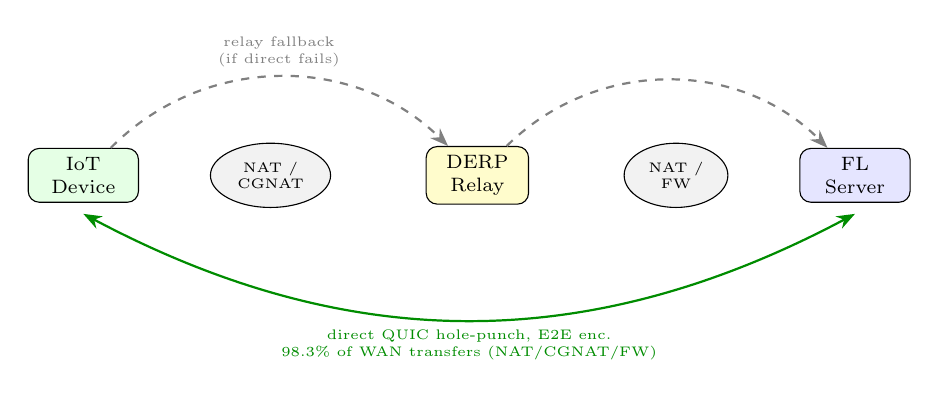
\begin{tikzpicture}[
    node distance=0.5cm,
    dev/.style={draw, rounded corners, fill=white, minimum width=1.4cm, minimum height=0.65cm, align=center, font=\scriptsize},
    nat/.style={draw, ellipse, fill=gray!10, minimum width=1.3cm, minimum height=0.6cm, align=center, font=\tiny},
    rly/.style={draw, rounded corners, fill=yellow!20, minimum width=1.3cm, minimum height=0.65cm, align=center, font=\scriptsize},
    >=Stealth]
  \node[dev, fill=green!10] (A) {IoT\\Device};
  \node[nat, right=0.9cm of A] (NA) {NAT /\\CGNAT};
  \node[rly, right=1.2cm of NA] (R) {DERP\\Relay};
  \node[nat, right=1.2cm of R] (NB) {NAT /\\FW};
  \node[dev, fill=blue!10, right=0.9cm of NB] (B) {FL\\Server};
  \draw[->, thick, gray, dashed, bend left=45] (A) to
    node[above, font=\tiny, align=center]{relay fallback\\(if direct fails)} (R);
  \draw[->, thick, gray, dashed, bend left=45] (R) to (B);
  \draw[<->, thick, green!55!black] ([yshift=-4pt]A.south) to[bend right=28]
    node[below, font=\tiny, green!55!black, align=center]{direct QUIC hole-punch, E2E enc.\\98.3\% of WAN transfers (NAT/CGNAT/FW)} ([yshift=-4pt]B.south);
\end{tikzpicture}
\caption{NAT traversal in FL-Iroh. Direct QUIC hole-punching is attempted first and, in our WAN tests, succeeds even under CGNAT and port-443 firewalls (green, end-to-end encrypted). The DERP relay remains a guaranteed fallback (grey dashed), used only if a direct path cannot be formed; the application is unaware of which path is active.}
\label{fig:holepunch}
\end{figure}

We address this gap with \textbf{FL-Iroh}, a system that integrates:

\begin{enumerate}
    \item \textbf{Iroh}~\cite{iroh2024}, a QUIC-based P2P transport library that implements the DERP relay protocol~\cite{tailscale2023}: hole-punching is attempted first; if it fails, all traffic is seamlessly relayed through a DERP server with end-to-end encryption---the application is unaware of the switchover.
    \item \textbf{CoAP/CoRE}~\cite{rfc7252} as a lightweight control plane for FL service discovery (resource directory, round coordination), using CBOR serialization for minimal overhead on constrained links.
    \item \textbf{FedAvg}~\cite{mcmahan2017} and \textbf{FedGAM} (selective aggregation of the shared seasonality coefficients of Generalized Additive Models, GAMs) as aggregation algorithms, operating over Iroh QUIC streams. The data plane is independent of IP addressing and, critically, \emph{algorithm-agnostic}: the same QUIC channel carries neural network weight tensors and Prophet Fourier coefficients without protocol modification.
\end{enumerate}

Our primary application domain is agricultural IoT: soil-based crop recommendation, where sensors measure N, P, K content, temperature, humidity, pH, and rainfall to recommend optimal crop selection. This represents a tabular inference task well-suited for lightweight MLP models on Cortex-A class edge devices (e.g., Raspberry Pi~4B), with potential for inference deployment on more constrained platforms.

\noindent\textbf{Contributions:}
\begin{enumerate}
    \item We design and implement FL-Iroh, an open-source, algorithm-agnostic FL architecture that embeds NAT traversal in the application-level transport---an Iroh\slash QUIC data plane with public-key peer addressing---coordinated by a lightweight CoAP\slash CBOR control plane (\S\ref{sec:system}). The NAT-traversal machinery itself is provided by the Iroh library~\cite{iroh2024}; our contribution is its integration into, and evaluation as, an FL substrate.
    \item We provide an empirical characterization of QUIC hole-punching and relay transport for FL workloads on real hardware (PC $\leftrightarrow$ Raspberry Pi across a 300~km WAN, different ISPs): every session connected, and 118 of 120 WAN transfers (98.3\%) used a direct hole-punched path---verified by active-path inspection---under full-cone NAT, symmetric NAT, CGNAT, and a port-443-only firewall, with the encrypted relay retained as a guaranteed fallback (\S\ref{sec:e3}).
    \item We conduct a six-experiment evaluation (E1--E6) plus an operational comparison with Flower-over-Tailscale, covering transport throughput, convergence under Non-IID heterogeneity, churn resilience, CoAP discovery scaling, and a two-domain application study: crop recommendation with a compact MLP (AgriMLP, 7.7K parameters) and seven-day-ahead air-quality forecasting (\S\ref{sec:evaluation}).
    \item We propose FedGAM, a partial-aggregation rule that federates only the shared seasonality coefficients of Prophet GAM models, and report an honest same-model ablation showing that, with eight years of local training data, FedGAM is statistically indistinguishable from FedAvg---delimiting the regime in which partial aggregation can matter (\S\ref{sec:e6}).
\end{enumerate}

The remainder of this paper is organized as follows. Section~\ref{sec:related} reviews related work. Section~\ref{sec:system} presents the FL-Iroh architecture, transport, control plane, and application models. Section~\ref{sec:evaluation} reports the experimental evaluation (E1--E6) and the operational comparison with Flower-over-Tailscale. Section~\ref{sec:discussion} discusses implications, the security model, and limitations. Section~\ref{sec:conclusion} concludes and outlines future work.

% =========================================================================
\section{Related Work}
\label{sec:related}

We organize prior work along five axes: FL in agriculture and environmental monitoring, NAT traversal, control planes for IoT ML, Non-IID mitigation, and alternative connectivity substrates (overlay VPNs and decentralized FL).

\subsection{Federated Learning for Agricultural and Environmental IoT}

FL has recently been applied across the agri-food sector. Durrant~et~al.~\cite{durrant2022} demonstrate cross-silo FL for collaborative data sharing among agricultural stakeholders, and Friha~et~al.~\cite{friha2022} propose a federated intrusion-detection system (FELIDS) for the agricultural Internet of Things. Device heterogeneity across farms---different soil types, crops, and microclimates---creates natural Non-IID distributions that challenge standard FedAvg~\cite{mcmahan2017}. Privacy is also a first-order concern: agronomic data (crop varieties, yields, fertilization schedules) are commercially sensitive and farmers are reluctant to share them. However, these works assume publicly reachable aggregation servers reached over conventional infrastructure (cross-silo data centres or pre-provisioned gateways); none addresses the NAT-traversal barrier that, in our experience, is a major practical obstacle to real-world agricultural FL deployment in rural environments with NAT/CGNAT. FL applications to outdoor air-quality monitoring---our second domain---remain scarce in the literature, which motivates the E6 study in this paper.

\subsection{NAT Traversal in P2P and IoT}

NAT traversal has been studied extensively since Ford et~al.'s foundational analysis of peer-to-peer communication across NATs~\cite{ford2005,rfc5128}, and underpins VoIP, WebRTC~\cite{webrtc2021}, and file-sharing systems. The STUN~\cite{rfc8489} and TURN~\cite{rfc8656} protocols provide the IETF foundations for hole-punching and relay fallback, and large-scale measurement campaigns in the libp2p ecosystem have characterized hole-punching success rates in the wild~\cite{seemann2022}. DERP (Designated Encrypted Relay for Packets), developed by Tailscale~\cite{tailscale2023}, provides an authenticated, encrypted, HTTPS-based relay that acts both as a rendezvous/signaling channel and as a relay of last resort---fulfilling the same architectural role as TURN, though it is not protocol-compatible with it---within the WireGuard VPN ecosystem. Iroh adapts DERP for general-purpose P2P applications~\cite{iroh2024}. In the IoT space, NGROK and similar tunneling services provide connectivity but introduce centralized dependencies and per-byte costs unsuitable for energy-constrained deployments.

\subsection{CoAP for FL Control Plane}

CoAP~\cite{rfc7252} (Constrained Application Protocol) provides a RESTful transfer protocol for constrained nodes and, together with the CoRE link format~\cite{rfc6690} and CBOR~\cite{rfc8949} (Concise Binary Object Representation) encoding, is a natural candidate for a lightweight \emph{control plane} for IoT ML pipelines, separating signaling (discovery, round coordination) from bulk data transfer. MQTT-based publish--subscribe signaling has also been used to coordinate distributed and federated training in IoT deployments; MQTT, however, lacks the RESTful resource model that enables semantic client filtering by sensor capability. To the best of our knowledge, no prior FL system combines a CoAP control plane with a NAT-traversing data-plane transport; CoAP-coordinated FL itself remains largely unevaluated. Our work uses CoAP exclusively as the control plane (registration, discovery, round signaling); model parameter transfer---the \emph{data plane}---occurs over Iroh/QUIC, which handles NAT traversal transparently and independently from the control channel.

\subsection{Non-IID FL in Resource-Constrained Environments}

Non-IID data is a well-studied challenge in FL~\cite{zhao2018noniid,li2022noniid,kairouz2021}. In agricultural settings, non-IID arises naturally from geographic heterogeneity: farms in different climate zones or with different soil types exhibit clearly distinct feature distributions. FedProx~\cite{fedprox2020} and SCAFFOLD~\cite{scaffold2020} mitigate gradient drift by regularizing against deviation from the global model, and client-clustering approaches group clients with similar local distributions before aggregation~\cite{briggs2020cluster}. For non-neural models---such as Prophet GAMs (Generalized Additive Models)---plain FedAvg is semantically questionable: it averages parameters whose local meanings differ across clients (e.g., the industrial emission trend of Ponferrada with the rural baseline of Soria). FL-Iroh explores FedGAM, which applies \emph{partial aggregation} over the shared seasonality coefficients only; our evaluation both demonstrates this design and, via a same-model ablation, delimits when it actually pays off (\S\ref{sec:e6}). We use Dirichlet $\alpha$ partitions as the standard Non-IID benchmark in E2.

\subsection{FL over Overlay and VPN Networks}

A pragmatic way to reach NATed devices is to place them on a shared overlay network. WireGuard~\cite{wireguard2017}-based meshes such as Tailscale~\cite{tailscale2023} and ZeroTier give every node a stable virtual IP and traverse NAT/CGNAT through the same DERP-style relays that Iroh uses, and have been adopted to interconnect distributed-ML and edge clusters. Relative to FL-Iroh, however, these approaches delegate connectivity to a separate system-level VPN daemon---typically requiring elevated privileges and an account-managed coordination server---while the FL framework itself (e.g., Flower~\cite{flower2022}) must still address a reachable server over a centralized star topology. FL-Iroh instead embeds NAT traversal in the application-level transport: peers are named by public key rather than by overlay IP, and no system VPN or persistent server address is required. We provide a qualitative operational comparison against Flower-over-Tailscale, together with an accuracy-parity check using a Flower-compatible harness, in \S\ref{sec:e7}.

\subsection{Decentralized and Serverless FL}

An orthogonal line of work removes the central aggregator altogether. Decentralized SGD trains over sparse communication graphs without a parameter server~\cite{lian2017}, gossip learning propagates and merges models epidemically among peers~\cite{hegedus2019}, and BrainTorrent demonstrates peer-to-peer FL without a central server in medical imaging~\cite{roy2019braintorrent}. These approaches address the aggregator as a statistical and topological bottleneck, but generally \emph{assume} that peers can reach one another---precisely the assumption that NAT and CGNAT break in the field. Production-oriented FL frameworks (Flower~\cite{flower2022}, FedML~\cite{fedml2020}, OpenFL~\cite{openfl2022}, NVIDIA FLARE~\cite{flare2022}) likewise assume a reachable coordination endpoint. FL-Iroh is complementary: it retains a logical aggregator (simplifying convergence semantics) while removing the requirement that any participant be publicly routable; because peers are addressed by public key, the same transport could also carry the fully decentralized topologies above.

% =========================================================================
\section{System Design}
\label{sec:system}

This section describes the FL-Iroh architecture (control and data planes), the Iroh transport and wire format, the CoAP control plane, and the application models used in the evaluation. Fig.~\ref{fig:agro} illustrates the target deployment: field sensors feed a Raspberry-Pi-class FL client that registers via CoAP and exchanges model parameters over Iroh/QUIC from behind NAT or CGNAT.

\subsection{Architecture Overview}

FL-Iroh is structured as two planes (Fig.~\ref{fig:architecture}):

\begin{itemize}
    \item \textbf{Control plane (CoAP/CoRE)}: A CoAP resource directory running on the FL aggregation node. Clients register their Iroh endpoint descriptors (node ID, addresses, relay URL) as CoAP resources on startup. The server discovers clients, manages round state, and disseminates lightweight round metadata (\texttt{round\_id}, \texttt{model\_hash}, server node ID) via CoAP GET/PUT with CBOR encoding; clients then fetch the model tensors over Iroh/QUIC (ALPN \texttt{fl-model/1}).
    \item \textbf{Data plane (Iroh/QUIC)}: All tensor data---model distributions (server$\to$client) and gradient uploads (client$\to$server)---flow over QUIC streams established by Iroh. Each QUIC stream carries a length-prefixed, SHA-256-verified payload. The ALPN protocol identifiers \texttt{fl-model/1} and \texttt{fl-update/1} distinguish model push from update upload.
\end{itemize}

\begin{figure}[t]
\centering
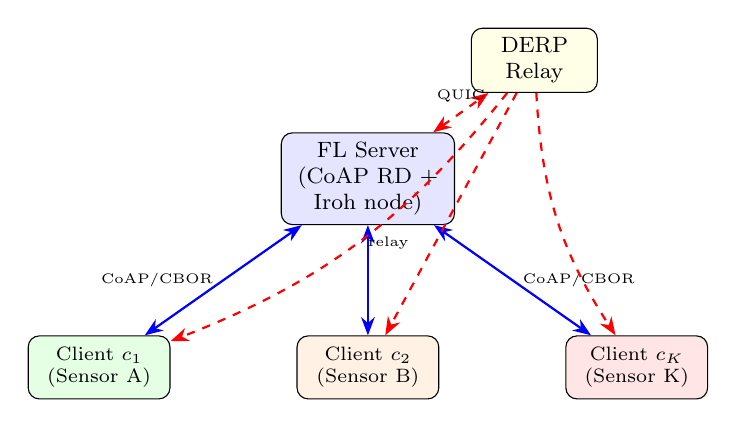
\begin{tikzpicture}[
    node distance=1.3cm and 1.0cm,
    box/.style={draw, rounded corners, minimum width=2.2cm, minimum height=0.9cm, align=center, font=\footnotesize},
    client/.style={draw, rounded corners, minimum width=1.8cm, minimum height=0.8cm, align=center, font=\scriptsize},
    plane/.style={draw, dashed, rounded corners, fill=gray!5, inner sep=4pt},
    >=Stealth
]
    \node[box, fill=blue!10] (srv) {FL Server\\(CoAP RD +\\Iroh node)};
    \node[client, below left=1.4cm and 1.4cm of srv, fill=green!10] (c1) {Client $c_1$\\(Sensor A)};
    \node[client, below=1.4cm of srv, fill=orange!10] (c2) {Client $c_2$\\(Sensor B)};
    \node[client, below right=1.4cm and 1.4cm of srv, fill=red!10] (ck) {Client $c_K$\\(Sensor K)};
    \node[box, above right=0.5cm and 0.2cm of srv, fill=yellow!10, minimum width=1.6cm, minimum height=0.7cm] (relay) {DERP\\Relay};
    \draw[<->, blue, thick] (srv) -- node[left, font=\tiny, black] {CoAP/CBOR} (c1);
    \draw[<->, blue, thick] (srv) -- (c2);
    \draw[<->, blue, thick] (srv) -- node[right, font=\tiny, black] {CoAP/CBOR} (ck);
    \draw[<->, red, thick, dashed] (srv) -- node[above, font=\tiny, black] {QUIC} (relay);
    \draw[->, red, thick, dashed, bend left=15] (relay) to node[right, font=\tiny, black] {relay} (c1);
    \draw[->, red, thick, dashed] (relay) -- (c2);
    \draw[->, red, thick, dashed, bend right=15] (relay) to (ck);
\end{tikzpicture}
\caption{FL-Iroh architecture. CoAP handles service discovery and round control (blue). Iroh/QUIC carries tensor data with transparent relay fallback (red dashed) when direct hole-punch fails.}
\label{fig:architecture}
\end{figure}

\begin{figure}[t]
\centering
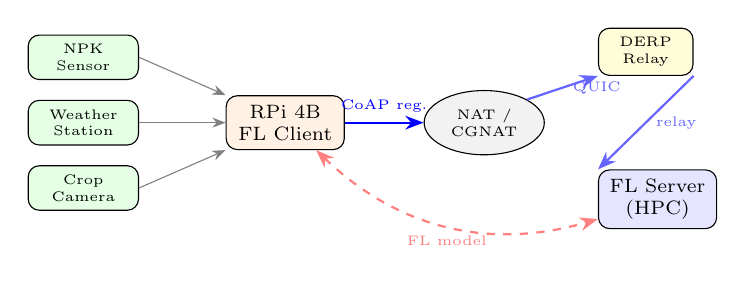
\begin{tikzpicture}[
    node distance=0.45cm and 0.35cm,
    sensor/.style={draw, rounded corners, fill=green!10, minimum width=1.4cm, minimum height=0.55cm, align=center, font=\tiny},
    edge/.style={draw, rounded corners, fill=orange!10, minimum width=1.5cm, minimum height=0.65cm, align=center, font=\scriptsize},
    srv/.style={draw, rounded corners, fill=blue!10, minimum width=1.5cm, minimum height=0.65cm, align=center, font=\scriptsize},
    rtr/.style={draw, ellipse, fill=gray!10, minimum width=1.2cm, minimum height=0.55cm, align=center, font=\tiny},
    rly/.style={draw, rounded corners, fill=yellow!15, minimum width=1.2cm, minimum height=0.55cm, align=center, font=\tiny},
    >=Stealth]
  \node[sensor] (s1) {NPK\\Sensor};
  \node[sensor, below=0.25cm of s1] (s2) {Weather\\Station};
  \node[sensor, below=0.25cm of s2] (s3) {Crop\\Camera};
  \node[edge, right=1.1cm of s2] (pi) {RPi 4B\\FL Client};
  \node[rtr, right=1cm of pi] (nat) {NAT /\\CGNAT};
  \node[rly, above right=0.3cm and 0.9cm of nat] (relay) {DERP\\Relay};
  \node[srv, below right=0.3cm and 0.9cm of nat] (srv) {FL Server\\(HPC)};
  \draw[->, gray, thin] (s1.east) -- (pi.north west);
  \draw[->, gray, thin] (s2.east) -- (pi.west);
  \draw[->, gray, thin] (s3.east) -- (pi.south west);
  \draw[->, blue, thick] (pi) -- node[above, font=\tiny]{CoAP reg.} (nat);
  \draw[->, blue!60, thick] (nat.north east) -- node[right, font=\tiny]{QUIC} (relay.south west);
  \draw[->, blue!60, thick] (relay.south east) -- node[right, font=\tiny]{relay} (srv.north west);
  \draw[<->, red!50, dashed, thick, bend right=30] (pi) to
    node[below, font=\tiny]{FL model} (srv);
\end{tikzpicture}
\caption{FL-Iroh deployment in agricultural IoT. Field sensors feed the FL client (Raspberry Pi), which registers via CoAP and exchanges model parameters over Iroh/QUIC with automatic fallback to DERP relay under NAT/CGNAT.}
\label{fig:agro}
\end{figure}

\subsection{Iroh Transport}

Iroh~\cite{iroh2024} creates a QUIC endpoint that embeds a \emph{node address} consisting of a 32-byte public key (node ID), a list of direct UDP addresses, and a DERP relay URL. When a client initiates a connection to another node, Iroh:
\begin{enumerate}
    \item Registers both parties with the DERP relay for signaling.
    \item Simultaneously attempts UDP hole-punching to each direct address.
    \item If hole-punching succeeds within a configurable timeout, the QUIC session migrates to the direct path.
    \item If no direct path can be negotiated (e.g., certain restrictive symmetric-NAT mappings), all QUIC packets are forwarded by the DERP relay transparently.
\end{enumerate}

FL-Iroh uses ALPN-based multiplexing: multiple protocol roles (model push, update upload) share a single Iroh node without port allocation.

\subsection{Wire Format}

Each QUIC unidirectional stream carries one tensor bundle:
\begin{equation}
\underbrace{[4\,\text{B}]}_{\text{len}} \;\; \underbrace{[\text{payload}]}_{\text{torch.save blob}} \;\; \underbrace{[32\,\text{B}]}_{\text{SHA-256}}
\label{eq:wire}
\end{equation}
The SHA-256 suffix provides integrity verification at the application layer, independent of QUIC's own encryption. The payload is serialized with \texttt{torch.save}, producing a self-describing binary format that handles mixed tensor types and dtypes.

\subsection{CoAP Control Plane}

The FL server exposes CoAP resources following the CoRE resource directory~\cite{rfc6690}:
\begin{itemize}
    \item \texttt{/fl/register}: Clients POST their Iroh endpoint JSON on startup.
    \item \texttt{/fl/round}: Server PUT triggers a new training round, carrying lightweight round metadata (\texttt{round\_id}, \texttt{model\_hash}, server node ID); clients fetch the global model tensors over Iroh/QUIC (ALPN \texttt{fl-model/1}).
    \item \texttt{/fl/discover}: Server queries registered clients with optional semantic filtering by capability tags (e.g., \texttt{sensor\_type=soil}).
\end{itemize}

CBOR~\cite{rfc8949} encoding reduces message overhead versus JSON by 30--50\% for numerical payloads, staying within 6LoWPAN block sizes for control messages.

\subsection{Application Models}

\textbf{AgriMLP} (Crop Recommendation). For the crop recommendation task, we use AgriMLP: a four-layer fully connected network (multilayer perceptron, MLP) with architecture $7 \to 64 \to 64 \to 32 \to 22$ (input features $\to$ output classes). The first two hidden layers use Batch Normalization and Dropout (rate~0.2) for regularization. Total trainable parameters: 7{,}734 ($\approx$31~KB at float32; $\approx$32~KB as a serialized state dict including normalization statistics), making it trivially deployable for on-device inference on Cortex-A class hardware (Raspberry Pi~4B, Jetson Nano). Input features are z-score normalized: soil macro-nutrients (N, P, K), temperature, humidity, pH, and rainfall.

\textbf{AirMLP} (7-Day-Ahead ICA Forecasting, Outdoor). For E6 we use AirMLP, a compact four-layer network $6 \to 32 \to 32 \to 16 \to 3$ (1{,}987 parameters, $\approx$8~KB at float32) with the same regularization scheme as AgriMLP. Inputs are daily outdoor measurements at time~$t$ (NO$_2$, O$_3$, particulate matter, CO) fused with meteorological predictors (wind speed and precipitation) from AEMET, the Spanish State Meteorological Agency, all z-score normalized. The task is to predict the ICA class (\'Indice de Calidad del Aire, the Spanish air-quality index) 7~days ahead ($t{+}7$); the full task definition, labeling scheme, and rationale are given in \S\ref{sec:e6}. This model applies to open-air monitoring stations only, not indoor or greenhouse installations.

\textbf{ProphetWrapper} (Federated GAM). FL-Iroh's transport layer is statistically model-agnostic: it serializes any \texttt{torch.state\_dict()} over Iroh/QUIC without interpreting parameter semantics. We exploit this to federate Facebook Prophet~\cite{taylor2018prophet}, a Generalized Additive Model (GAM), by wrapping it in an \texttt{nn.Module} adapter. The wrapper exposes a compatible \texttt{state\_dict()}/\texttt{load\_state\_dict()} interface that extracts and injects the Fourier seasonality coefficients (annual: $N{=}10$ sin/cos pairs; weekly: $N{=}3$) and the wind-speed regressor weight as floating-point tensors. Trend parameters ($k$, $m$, $\delta$) encode province-specific industrial and demographic emission patterns (e.g., Ponferrada coal plant vs.\ rural Soria) and are therefore \emph{not} federated; they remain local to each province client. This design, which we term \textbf{FedGAM}, federates only the shared periodic structure of pollutant cycles while preserving local trend identity---a separation consistent with the seasonal structure documented for this dataset in prior work~\cite{lopezblanco2024airquality}.

The current FL client requires Python~3.11 and PyTorch; porting to Cortex-M MCU-class platforms would require a C or Rust reimplementation of the client runtime.

% =========================================================================
\section{Experimental Evaluation}
\label{sec:evaluation}

We report six experiments (E1--E6) followed by an operational comparison with Flower-over-Tailscale (\S\ref{sec:e7}). Throughout, we distinguish two connectivity metrics: \emph{session-level establishment} (whether a usable connection is eventually formed, including retries) and the \emph{per-transfer direct-path rate} (the fraction of individual transfers carried over a hole-punched path rather than the relay).

\subsection{Experimental Setup}

All experiments run on a single-node HPC cluster (Intel Xeon, 16 cores, no GPU) for E2, E4, E5, E6, and on real hardware (PC with WSL2 + Raspberry Pi~4B, 300~km WAN separation) for E1 distributed and E3. FL experiments use $K{=}10$ clients with FedAvg (or FedGAM for E6-Prophet), $E{=}1$ local epoch per round, SGD optimizer (lr$=$0.01), and $R{=}100$ global rounds for E2 and E4, $R{=}50$ for E6. E2 uses SimpleCNN, a three-block convolutional network (Conv--BN--ReLU blocks of 32/64/128 channels with max-pooling, global average pooling, and a linear head; 94{,}762 trainable parameters, $\approx$0.38~MB serialized state dict) on CIFAR-10~\cite{cifar2009}. The Crop Recommendation dataset~\cite{cropdataset} contains 2,200 records across 22 crop classes (100 records/class), partitioned using Dirichlet allocation with concentration $\alpha \in \{0.1, 0.5, 1.0\}$ and IID as a baseline. The E6 air quality dataset covers 10 Castilla y Le\'on monitoring zones---the nine provincial capitals plus Ponferrada---over 2011--2019 (train: 2011--2018, test: 2019) with a geographic partition (one client per zone) and an IID shuffled baseline. Multi-seed runs use a fixed replication-seed registry ($n{=}5$ seeds); 95\% confidence intervals use the Student-$t$ distribution. Code and data are available at \url{https://github.com/raullb34/FL-Iroh}.

\subsection{E1: Transport Throughput}
\label{sec:e1}

We benchmark three transport configurations across four payload sizes (100~KB, 1~MB, 10~MB, 100~MB):

\begin{itemize}
    \item \textbf{HTTP/2 (loopback)}: aiohttp server+client on localhost, serving as a ceiling baseline.
    \item \textbf{iroh\_relay\_loopback}: Two in-process Iroh nodes on the same machine, using the public DERP relay \texttt{euw1-1.relay.iroh.network}.
    \item \textbf{iroh\_relay\_wan}: PC as server and Raspberry Pi~4B (300~km geographic separation, different ISPs) as client, using the same public DERP relay. The separation ensures no shared routing infrastructure, representing a realistic worst-case WAN scenario.
\end{itemize}

Results are shown in Table~\ref{tab:e1}. HTTP/2 peaks at 573~Mbps for 1~MB payloads on loopback, dropping to 244~Mbps at 100~MB (memory bandwidth limited). The iroh relay loopback achieves 27.2~Mbps at 100~KB ($N{=}14$, preliminary), reflecting QUIC+relay encryption overhead on a fast local path. The WAN relay saturates at 2.8~Mbps independent of payload size ($N{=}30$ per cell). For AgriMLP model exchanges ($\approx$31~KB per direction), transport time over the WAN relay is $\approx$110~ms per push and $\approx$220~ms for a full download-plus-upload exchange, yielding $<$1~s per federated round at the network level. Note that Table~\ref{tab:e1} characterizes the \emph{relay} path, which E3 shows to be the uncommon fallback case; direct hole-punched paths avoid the relay hop entirely and are bounded by the end-to-end link capacity instead.

\begin{table}[t]
\centering
\caption{E1: Transport Throughput Summary}
\label{tab:e1}
\footnotesize
\setlength{\tabcolsep}{4pt}
\resizebox{\columnwidth}{!}{%
\begin{tabular}{l r r r r}
\toprule
\textbf{Transport} & \textbf{Payload} & \textbf{Mean (Mbps)} & \textbf{P95 (Mbps)} & \textbf{N} \\
\midrule
HTTP/2               & 100~KB  & 208.2  & 245.5  & 30 \\
HTTP/2               & 1~MB    & 573.6  & 603.3  & 30 \\
HTTP/2               & 10~MB   & 479.2  & 560.3  & 30 \\
HTTP/2               & 100~MB  & 244.6  & 248.9  & 30 \\
\midrule
iroh relay loopback  & 100~KB  & 27.2   & 29.2   & 14 \\
\midrule
iroh relay WAN       & 100~KB  & 2.26   & 2.43   & 30 \\
iroh relay WAN       & 1~MB    & 2.75   & 2.79   & 30 \\
iroh relay WAN       & 10~MB   & 2.81   & 2.82   & 30 \\
iroh relay WAN       & 100~MB  & 2.81   & 2.83   & 30 \\
\bottomrule
\end{tabular}%
}
\end{table}

The flat throughput curve across payloads (100~KB to 100~MB all saturate at $\approx$2.8~Mbps, $N{=}30$ per cell, stdev${<}$0.05~Mbps) points to a relay-side ceiling---server capacity or per-connection rate limiting on the public relay---rather than QUIC protocol overhead; we did not benchmark a self-hosted DERP relay to separate the two explanations. Either way, a self-hosted relay on a dedicated server would lift this ceiling, and the public relay already suffices for AgriMLP-sized model updates ($\approx$220~ms per round-trip exchange).

\subsection{E2: FL Convergence Under Non-IID Data}
\label{sec:e2}

We evaluate FedAvg convergence on CIFAR-10 with SimpleCNN under IID and non-IID (Dirichlet $\alpha{=}0.1$) partitioning. All runs use $K{=}10$ clients, $E{=}1$ local epoch, cross-entropy loss, SGD optimizer (lr$=$0.01), $R{=}100$ rounds. Multi-seed replication ($n{=}5$) provides 95\% confidence intervals via Student-t distribution. Results in Table~\ref{tab:e2}.

\begin{table}[t]
\centering
\caption{E2: FL Convergence on CIFAR-10 (SimpleCNN, $K{=}10$, $R{=}100$, $n{=}5$ seeds)}
\label{tab:e2}
\footnotesize
\begin{tabular}{l r r}
\toprule
\textbf{Partition} & \textbf{Test Acc. (final)} & \textbf{95\% CI} \\
\midrule
IID                  & 65.86\% & [65.66\%, 66.06\%] \\
Dirichlet $\alpha{=}0.1$ & 44.18\% & [39.45\%, 48.92\%] \\
\bottomrule
\end{tabular}
\end{table}

Under IID partitioning, SimpleCNN converges to 65.86\% test accuracy with a tight 95\% CI of $\pm$0.2pp ($n{=}5$ seeds), demonstrating reproducible convergence. Severe non-IID heterogeneity (Dirichlet $\alpha{=}0.1$) causes substantial degradation to 44.18\%, with a wider CI of $\pm$4.7pp reflecting increased variance across different client-data assignments. The 21.7pp accuracy gap quantifies the cost of label skew in CIFAR-10 FL, consistent with prior work~\cite{li2020federated,scaffold2020}. Despite heterogeneity, FedAvg converges without divergence, validating the robustness of the transport layer under realistic non-IID conditions.

A heterogeneity sweep over the Dirichlet concentration parameter (single-seed runs) confirms the expected monotonic trend: accuracy degrades smoothly from IID (65.86\%) through $\alpha{=}1.0$ (63.95\%) and $\alpha{=}0.5$ (62.64\%) to the severe $\alpha{=}0.1$ regime, where label skew becomes the dominant error source. The transport layer imposes no additional convergence penalty at any heterogeneity level: all runs complete their full 100 rounds with 100\% round-level success and an identical per-round byte cost of 3.87~MB of aggregated client updates ($K{=}10$ updates $\times$ $\approx$0.387~MB serialized SimpleCNN state dict each).

\subsection{E3: NAT Traversal Success Rate}
\label{sec:e3}

We measure connection establishment success and, where the transport API exposes it, the connection type (direct hole-punch vs.~relay) across five network scenarios using real hardware:

\begin{itemize}
    \item \textbf{net\_lan}: both peers on the same local network (control baseline).
    \item \textbf{net\_nat1} (full-cone NAT): PC behind a standard home router (Spain) $\leftrightarrow$ Raspberry Pi~4B (remote location, 300~km).
    \item \textbf{net\_nat2} (symmetric NAT): a second NAT topology with a different router pairing.
    \item \textbf{net\_cgnat} (Carrier-Grade NAT): same hardware, with the PC behind an ISP-level CGNAT.
    \item \textbf{net\_fw443} (restrictive firewall): outbound traffic constrained to port~443 only.
\end{itemize}

Each scenario runs $N{=}30$ transfers over a single established session (1--3 distinct QUIC connections per run), so the unit of analysis in Table~\ref{tab:e3} is the \emph{transfer}, not an independent connection-establishment attempt: across the four WAN scenarios the 120 transfers correspond to roughly 4--12 distinct QUIC connections on one PC$\leftrightarrow$Raspberry~Pi hardware pair. Transfer-level percentages therefore measure the stability of the direct path during operation; they should not be read as a population-level hole-punching success probability (see \S\ref{sec:limitations}). Results are shown in Table~\ref{tab:e3}.

\begin{table*}[t]
\centering
\caption{E3: NAT Traversal Results ($N{=}30$ transfers per scenario, one established session each; connection path classified via Iroh \texttt{remote\_info()} active-path inspection)}
\label{tab:e3}
\footnotesize
\begin{tabular}{l r r r r l}
\toprule
\textbf{Scenario} & \textbf{$N$} & \textbf{Direct (\%)} & \textbf{Relay (\%)} & \textbf{Failed (\%)} & \textbf{Active path} \\
\midrule
net\_lan   (LAN baseline)   & 30 & 100.0 & 0.0 & 0.0 & direct (local)  \\
net\_nat1  (full-cone NAT)  & 30 & 96.7  & 0.0 & 3.3 & direct (public) \\
net\_nat2  (symmetric NAT)  & 30 & 100.0 & 0.0 & 0.0 & direct (public) \\
net\_cgnat (CGNAT)          & 30 & 96.7  & 0.0 & 3.3 & direct (public) \\
net\_fw443 (firewall :443)  & 30 & 100.0 & 0.0 & 0.0 & direct (public) \\
\midrule
\textbf{WAN aggregate}      & 120 & \textbf{98.3} & \textbf{0.0} & 1.7 & direct (public) \\
\bottomrule
\end{tabular}
\end{table*}

The key result: direct QUIC hole-punching carried every completed WAN transfer in every NAT, CGNAT, and firewall scenario---with 0\% relay usage. Of 120 WAN transfers (four scenarios $\times$ 30), 118 (98.3\%) rode a \emph{direct} peer-to-peer path and none fell back to the DERP relay; the two failures (1.7\%) were first-attempt cold-start timeouts that succeeded on retry within the same session, so session-level establishment was 100\%. In every direct connection the active wire address was the remote peer's \emph{public} IP, not a private LAN address---confirming a genuine hole-punched WAN path rather than a co-located shortcut. For the CGNAT scenario we additionally verified network isolation by confirming the two peers' private subnets were mutually unreachable (100\% packet loss), with the PC on a mobile-carrier CGNAT and the Raspberry Pi 300~km away on a different fixed ISP. Direct connectivity thus held even under Carrier-Grade NAT, symmetric NAT, and a port-443-only firewall, cross-ISP. As a control, the same-LAN baseline (net\_lan, both peers co-located) instead reported the peer's \emph{private} RFC1918 address with sub-50~ms latency (15--47~ms vs.~62--625~ms over WAN), confirming that the active-path classifier faithfully distinguishes a local direct path from a WAN hole-punched one rather than defaulting to a public address.

Connection establishment (cold start) is variable---from 5.3~s (CGNAT) to 113~s (symmetric NAT)---while the direct path and relay candidates are negotiated and the NAT mapping is discovered; once established, steady-state transfer latency is low (62--625~ms, typically $<$300~ms), and subsequent transfers reuse the direct path. These latencies are acceptable for FL model exchange, where local training dominates round time.

This result is stronger than the relay-fallback guarantee alone: Iroh's hole-punching formed direct paths even under the symmetric-NAT and CGNAT conditions that classically defeat it. The DERP relay remains a \emph{guaranteed} fallback---ensuring connectivity by construction when a direct path cannot be formed---but was not exercised in any trial. Two caveats bound the generality of this finding: the measurements come from a single hardware pair over one pairing of ISPs, and the scenario labels reflect the deployed router/ISP configurations---we did not independently classify each NAT's mapping and filtering behavior with RFC~4787-style STUN probes, so ``symmetric NAT'' describes the configured topology rather than a verified mapping type. The evaluation is nonetheless a conservative setting: two peers with no shared routing infrastructure, on different ISPs 300~km apart, stressed by CGNAT and port restrictions.

\paragraph{Repeated cold-start establishment.}
The transfer-level percentages in Table~\ref{tab:e3} measure the stability of an already-established path but do not estimate how often an \emph{independent} cold start succeeds. To close this gap we ran a dedicated campaign: for each scenario we performed $N{=}30$ fully independent connection attempts, each spawning a fresh process with a new Iroh endpoint and a new NAT-mapping discovery, with a pause between attempts so that NAT mappings expire. This yields 30 independent cold-start establishment events per scenario---150 in total---the unit of analysis missing from Table~\ref{tab:e3}. Results are shown in Table~\ref{tab:e3est}. Across all 150 cold starts, 145 established a connection on the first attempt (96.7\%) and \emph{every} established connection used a \emph{direct} hole-punched path---the DERP relay was selected in 0 of 150 attempts. Restricted to the four WAN scenarios (120 attempts), 116 established directly (96.7\%); the five failures overall (three under CGNAT, one under symmetric NAT, one under the LAN profile) were first-attempt cold-start timeouts, consistent with the transient timeouts seen at the transfer level, and none fell back to the relay. In every established connection the active wire address was the peer's \emph{public} IP, confirming genuine hole-punched WAN paths on this cross-ISP pair for all five netem profiles (in this campaign the client ran remotely, so even the LAN profile physically traversed the WAN). Median establishment time was 0.4--1.4~s per scenario, with occasional multi-second tails (up to 77~s under symmetric NAT) reflecting variable NAT-mapping negotiation during a cold start; once established, steady-state transfers reuse the direct path. This connection-level evidence corroborates and strengthens the transfer-level result: direct hole-punching is not only stable once formed but is reached on the first cold-start attempt in the large majority of independent trials, with the encrypted relay retained as a guaranteed---though in practice unexercised---fallback.

\begin{table*}[t]
\centering
\caption{E3 (extended): repeated independent cold-start connection establishment ($N{=}30$ attempts per scenario; each attempt is a fresh process with a new Iroh endpoint and NAT-mapping discovery; path classified via Iroh \texttt{remote\_info()} active-path inspection). Median est.\ = median establishment time of the successful direct cold starts.}
\label{tab:e3est}
\footnotesize
\begin{tabular}{l r r r r r r}
\toprule
\textbf{Scenario} & \textbf{Attempts} & \textbf{Direct} & \textbf{Relay} & \textbf{Failed} & \textbf{Direct (\%)} & \textbf{Median est.} \\
\midrule
net\_lan   (LAN profile)    & 30  & 29  & 0 & 1 & 96.7  & 415~ms  \\
net\_nat1  (full-cone NAT)  & 30  & 30  & 0 & 0 & 100.0 & 453~ms  \\
net\_nat2  (symmetric NAT)  & 30  & 29  & 0 & 1 & 96.7  & 391~ms  \\
net\_cgnat (CGNAT)          & 30  & 27  & 0 & 3 & 90.0  & 439~ms  \\
net\_fw443 (firewall :443)  & 30  & 30  & 0 & 0 & 100.0 & 1411~ms \\
\midrule
\textbf{WAN aggregate}      & 120 & \textbf{116} & \textbf{0} & 4 & \textbf{96.7} & 522~ms \\
\textbf{All scenarios}      & 150 & \textbf{145} & \textbf{0} & 5 & \textbf{96.7} & 503~ms \\
\bottomrule
\end{tabular}
\end{table*}

\subsection{E4: Churn Resilience}
\label{sec:e4}

Agricultural IoT devices are subject to intermittent connectivity: power outages, cellular signal drops, and device maintenance cause clients to drop mid-round. We simulate churn by randomly dropping $p \in \{0, 10, 30, 50\}$\% of clients per round. FedAvg aggregates only the updates received in each round, with no special handling for missing clients. Table~\ref{tab:e4} reports final and peak accuracy, an early-convergence marker (the first round at which test accuracy exceeds 40\%), and round completion. Each configuration is a single run; differences below one percentage point between rows should not be over-interpreted.

\begin{table*}[t]
\centering
\caption{E4: Churn Resilience (Crop Recommendation, IID, $R{=}100$)}
\label{tab:e4}
\footnotesize
\begin{tabular}{l r r r r}
\toprule
\textbf{Churn rate} & \textbf{Acc (final)} & \textbf{Acc (max)} & \textbf{Rounds$\to$40\%} & \textbf{Completed rounds} \\
\midrule
0\%  & 93.18\% & 93.18\% & 16 & 100/100 \\
10\% & 92.95\% & 93.86\% & 17 & 100/100 \\
30\% & 93.64\% & 94.32\% & 16 & 100/100 \\
50\% & 93.64\% & 93.64\% & 18 & 100/100 \\
\bottomrule
\end{tabular}
\end{table*}

Accuracy remains stable at 93.2--93.6\% across all churn rates, with no meaningful degradation even at 50\% dropout. All 100 training rounds complete in every configuration. This robustness arises from two factors: (i) FedAvg aggregation tolerates partial participation---the server aggregates whichever client updates arrive each round, and (ii) with IID data distribution the gradient contributions from any subset of clients remain representative of the global distribution.

Note that churn is simulated by probabilistically withholding clients from each round (in-process, no actual network disconnection). In a real deployment, Iroh's relay-fallback ensures that reconnecting clients can always reach the server even after their IP address or NAT mapping has changed, so the partial-participation model is an accurate proxy for transient dropout.

\subsection{E5: CoAP Discovery Overhead}
\label{sec:e5}

Service discovery is a prerequisite for FL: each round, the server must locate available clients. We measure CoAP discovery latency and response size as a function of network size $N_{\text{nodes}} \in \{10, 50, 100\}$ and filter type:

\begin{itemize}
    \item \textbf{None filter}: Returns all registered endpoints (no filtering).
    \item \textbf{Semantic filter}: Filters endpoints by sensor capability tag (e.g., soil type), requiring string matching over resource descriptions.
\end{itemize}

\begin{table}[t]
\centering
\caption{E5: CoAP Discovery Overhead}
\label{tab:e5}
\footnotesize
\resizebox{\columnwidth}{!}{%
\begin{tabular}{r l r r r r}
\toprule
\textbf{N nodes} & \textbf{Filter} & \textbf{Mean (ms)} & \textbf{P95 (ms)} & \textbf{Bytes} & \textbf{N} \\
\midrule
10  & none     & 1.6  & 1.9  & 250   & 30 \\
10  & semantic & 24.0 & 26.4 & 2500  & 30 \\
50  & none     & 1.9  & 2.1  & 250   & 30 \\
50  & semantic & 130.7 & 156.6 & 12500 & 30 \\
100 & none     & 1.9  & 2.2  & 250   & 30 \\
100 & semantic & 278.7 & 344.1 & 25000 & 30 \\
\bottomrule
\end{tabular}%
}
\end{table}

Table~\ref{tab:e5} summarizes the results. The none filter achieves constant latency ($\approx$1.9~ms) and bandwidth (250~bytes) regardless of network size---O(1) \emph{by design}, since the server returns only active-round participants without iterating all resources. The semantic filter, which is the realistic discovery operation when selecting clients by capability, shows the expected O(n) scaling: 24~ms/2500~B at 10 nodes, growing to 278~ms/25000~B at 100 nodes---approximately 2.8~ms and 250~bytes per additional node. For typical agricultural deployments with $<$50 devices per farm cluster, semantic discovery completes in $<$157~ms, acceptable as a round-setup step executed once per FL round.

\emph{Note on byte estimates}: Discovery latency is measured by issuing $N_\text{nodes}$ actual CoAP GET requests per iteration. Reported byte counts for the semantic-filter rows are extrapolated as $250\,\text{B} \times N_\text{nodes}$ from the per-node measurement; real multi-server deployments may differ by a small constant factor due to CoAP framing.

\subsection{E6: Air Quality Federated Learning}
\label{sec:e6}

\textbf{Dataset and Task.} We use the Castilla y Le\'on historical daily air quality archive~\cite{cyl2023airquality} (1997--2020, 10 provinces), merged with AEMET~\cite{aemet2023} meteorological data (wind speed, precipitation). We restrict to 2011--2019 to avoid the COVID-19 lockdown artefact (anomalously low NO$_2$ in March--May~2020 documented in~\cite{lopezblanco2024airquality}). Train: 2011--2018; test: 2019.

The prediction task is \textbf{7-day-ahead ICA forecasting}: given outdoor sensor readings at day~$t$ (NO$_2$, O$_3$, PM, CO, wind speed, precipitation), predict the ICA air quality class 7~days ahead ($t{+}7$). This horizon is actionable for agricultural planning: a farmer observes today's readings and receives a weekly outlook for outdoor air quality risk (e.g., to schedule open-field spraying or harvest operations). The 7-day shift also eliminates the target-leakage that would arise from classifying the same-day NO$_2$ value that is also present as a feature.

ICA labels use training-set NO$_2$ terciles ($T_1{=}7.5$, $T_2{=}13.0~\mu$g/m$^3$) for 3-class targets that are balanced \emph{in-sample}: \textit{Bajo}~(low), \textit{Medio}~(medium), \textit{Alto}~(high). This replaces the absolute Spanish ICA thresholds (40/100~$\mu$g/m$^3$), which are designed for hourly peaks and produce a 99\%+ single-class imbalance on daily medians. The tercile approach preserves the NO$_2$ ranking and yields geographically non-IID distributions: industrial Valladolid has 73\% \textit{Alto} days vs.\ 18\% for rural Soria. Because the terciles are fitted on 2011--2018 training data and NO$_2$ levels declined over the decade, the held-out 2019 test year is \emph{not} balanced: its class distribution is 49.3\% \textit{Bajo}, 27.8\% \textit{Medio}, 22.9\% \textit{Alto}. Trivial baselines must therefore be computed on the test year rather than assumed from the in-sample balance; we report them in Table~\ref{tab:e6}.

\textbf{Deployment scope.} The feature set includes outdoor meteorological variables (AEMET wind speed, precipitation). This dataset applies to \emph{outdoor} monitoring installations; greenhouse or indoor deployments require a different feature set (removing wind/precipitation, adding CO$_2$, humidity). The 10 monitoring-zone clients are: \'Avila, Burgos, Le\'on, Palencia, Ponferrada, Salamanca, Segovia, Soria, Valladolid, and Zamora (the nine provincial capitals plus Ponferrada). Sensor tags are registered via CoAP with the \texttt{rt=air-quality} attribute.

\textbf{Configurations.} We run six configurations to isolate model and aggregation effects: AirMLP + FedAvg (geographic and IID), ProphetWrapper + FedGAM, and ProphetWrapper + FedAvg (geographic and IID). Multi-seed replication ($n{=}5$) provides 95\% confidence intervals.

\begin{table}[t]
\centering
\caption{E6: 7-Day-Ahead ICA Forecasting ($K{=}10$, $R{=}50$, test 2019, $n{=}5$ seeds)}
\label{tab:e6}
\footnotesize
\resizebox{\columnwidth}{!}{%
\begin{tabular}{l l r r}
\toprule
\textbf{Model} & \textbf{Partition} & \textbf{Test Acc.} & \textbf{95\% CI} \\
\midrule
Majority class (train)      & ---        & 22.94\% & (deterministic) \\
Persistence (class at $t{-}7$) & ---     & 47.54\% & (deterministic) \\
\midrule
AirMLP (FedAvg)             & Geographic & 47.26\% & [46.38\%, 48.14\%] \\
AirMLP (FedAvg)             & IID        & 49.63\% & [49.08\%, 50.17\%] \\
\midrule
ProphetWrapper (FedGAM)     & Geographic & 56.78\% & (deterministic) \\
ProphetWrapper (FedGAM)     & IID        & 57.93\% & [57.31\%, 58.55\%] \\
ProphetWrapper (FedAvg)     & Geographic & 56.59\% & (deterministic) \\
ProphetWrapper (FedAvg)     & IID        & 57.66\% & [57.26\%, 58.06\%] \\
\bottomrule
\end{tabular}%
}
\vspace{0.5em}

\emph{7-day-ahead ICA forecasting on outdoor CyL stations, test year 2019 (class distribution 49.3/27.8/22.9\%; labels from training-set NO$_2$ terciles $T_1{=}7.5$, $T_2{=}13.0~\mu$g/m$^3$, balanced in-sample only). Trivial baselines: majority class fitted on train (\textit{Alto}) and 7-day persistence (predict the class observed at $t{-}7$; 3,551 of 3,561 test rows have the $t{-}7$ observation available). Geographic non-IID: 10 natural zone partitions. Prophet geographic runs are deterministic MAP fits: the five seeds coincide, so no meaningful CI exists (effectively $n{=}1$). Accuracy values are on the held-out 2019 test set.}
\end{table}

\textbf{Trivial baselines.} Two deterministic baselines calibrate the difficulty of the task on the 2019 test year. A majority-class predictor fitted on the training data (\textit{Alto}) achieves only 22.94\%---\emph{below} the nominal 33.3\% of a balanced random guess---because the class distribution shifts between the training window and 2019. The stronger trivial baseline is 7-day \emph{persistence} (predict for $t{+}7$ the class observed at $t$), the canonical reference in forecasting, which achieves 47.54\%.

\textbf{AirMLP + FedAvg.} The 7-day-ahead ICA forecasting task is intrinsically hard for a memoryless MLP: the model receives a single day's measurements at time~$t$ and must predict the ICA class 7~days later, without access to the intervening trajectory. AirMLP reaches 49.63\% accuracy (IID, 95\% CI [49.08\%, 50.17\%]) and 47.26\% (geographic, [46.38\%, 48.14\%]). Measured against the persistence baseline, AirMLP-IID improves by only $+$2.1pp and the geographic configuration is statistically indistinguishable from persistence---the memoryless MLP essentially matches, but does not beat, the trivial forecaster. Its role in this study is therefore that of a reproducible, low-resource \emph{system} baseline (it exercises the FL transport with realistic tensors), not a competitive forecasting model. The 2.4pp gap between IID and geographic partitions confirms that zone-level non-IID costs accuracy---Ponferrada (industrial, coal-fired) vs.~rural Soria exhibit different NO$_2$ distributions---though FedAvg converges without divergence.

\textbf{ProphetWrapper: FedGAM vs. FedAvg Ablation.} Prophet GAM models reach 57.93\% (IID) and 56.78\% (geographic) with FedGAM---$+$10.4pp over the persistence baseline and $+$8.3/$+$9.5pp over AirMLP---making the Prophet configurations the only ones that clearly beat the trivial forecaster. Critically, the same-model ablation Prophet+FedAvg yields 57.66\% (IID) and 56.59\% (geographic)---statistically indistinguishable from FedGAM (Welch $p{=}0.35$ for IID, $\Delta{<}0.3$pp for geographic, $n{=}5$ seeds). This confirms that \emph{the model family, not the aggregation rule}, drives the accuracy gain: Prophet's internal Fourier decomposition captures NO$_2$ seasonality that a memoryless MLP cannot. FedGAM's partial aggregation (federating only seasonality coefficients, keeping trend parameters local) offers no measurable advantage over naive FedAvg on this task, likely because 8 years of training data provides sufficient local trend estimation even without federation. The geographic Prophet runs are deterministic MAP fits (all seeds coincide, effectively $n{=}1$), so their reported values carry no seed-level uncertainty estimate.

\textbf{Algorithm-Agnosticism of FL-Iroh.} Switching from FedAvg to FedGAM requires a single server-side change: \texttt{aggregator\_fn=fedgam\_aggregate}. The Iroh/QUIC data plane is oblivious to parameter semantics---it serializes any \texttt{torch.state\_dict()} as a binary blob and delivers it to each client unchanged. The same Iroh channels that carried AirMLP weight tensors (1{,}987 parameters, $\approx$8~KB) also carry ProphetWrapper Fourier tensors (27 parameters, $<$1~KB) without protocol modification. This is the central claim of FL-Iroh: \emph{the transport does not constrain the algorithm}. Operators can deploy domain-specific aggregation strategies---FedGAM for GAMs, FedProx for heterogeneous neural networks, partial aggregation for gradient-boosted trees---on existing IoT networks without touching the connectivity layer.

\subsection{Operational Comparison with Flower over Tailscale}
\label{sec:e7}

The closest deployable alternative to FL-Iroh for NAT-constrained FL is to run a conventional framework (Flower~\cite{flower2022}) over a WireGuard mesh VPN such as Tailscale~\cite{tailscale2023}, which gives every node a stable virtual IP and traverses NAT\slash CGNAT through DERP-style relays. Both stacks ultimately rely on relay-assisted NAT traversal and end-to-end encryption; the difference is \emph{where} connectivity lives. Table~\ref{tab:e7} contrasts the two along eight operational axes. The comparison is primarily architectural, but we also empirically verify accuracy parity (Table~\ref{tab:e7acc}): because both stacks run identical FL algorithms, the distinguishing factors are deployment surface, external dependencies, and operational cost rather than statistical performance.

\begin{table*}[t]
\centering
\caption{FL-Iroh vs.\ Flower-over-Tailscale operational comparison}
\label{tab:e7}
\footnotesize
\renewcommand{\arraystretch}{1.25}
\setlength{\tabcolsep}{4pt}
\begin{tabular}{p{2.4cm} p{6.2cm} p{6.2cm}}
\toprule
\textbf{Axis} & \textbf{FL-Iroh} & \textbf{Flower + Tailscale} \\
\midrule
NAT / CGNAT traversal & Built-in: QUIC hole-punching with transparent DERP relay fallback (E2E encrypted) & Delegated to the Tailscale overlay (WireGuard + DERP); Flower itself still needs a reachable server address \\
Server reachability & Peer addressed by 32-byte public node ID; no routable server IP required & Clients must know the server's Tailnet IP (100.x.y.z); centralized star topology \\
External infrastructure & Public or self-hosted DERP relay only (stateless, swappable) & Tailscale coordination server (control plane) $+$ DERP $+$ long-lived FL server process \\
Extra system daemon & None---userspace library, no elevated privileges & \texttt{tailscaled} system daemon on every node (typically root / \texttt{NET\_ADMIN}) \\
Transport encryption & End-to-end QUIC/TLS~1.3 (relay sees only ciphertext) & End-to-end WireGuard (relay sees only ciphertext) \\
Manual setup per node & Exchange node IDs (one out-of-band value) & Install \texttt{tailscaled}, authenticate node to tailnet, discover server IP, open/forward port \\
Topology & P2P data plane $+$ CoAP control plane; no routable server IP required & Centralized star; the FL server is a single point of failure \\
Account / ToS dependency & No account; default public relay operated by n0 (subject to its terms), fully self-hostable & Tailscale account $+$ ACL policy management (free-tier device/user caps) \\
\bottomrule
\end{tabular}
\end{table*}

\paragraph{Accuracy parity.}
To confirm that the choice of transport does not affect model quality, we ran the identical FedAvg workload (SimpleCNN on CIFAR-10, $K{=}10$ clients, $R{=}100$ rounds, $n{=}5$ seeds using the same replication seeds as E2) through a Flower-compatible reference harness---an \emph{in-process simulation} that reuses the same model, partitions, and training loop, not a live Flower deployment over a Tailscale mesh---and compared final test accuracy against FL-Iroh's E2 measurements (Table~\ref{tab:e7acc}). Under both IID and severe non-IID ($\alpha{=}0.1$) partitions the two stacks are statistically indistinguishable---each mean lies within the other's 95\% CI. This parity is expected by construction (both run FedAvg with identical hyperparameters and seeds); it serves as a sanity check that FL-Iroh's P2P data plane introduces no accuracy artifact, not as evidence of operational superiority. Quantitative operational measurements of a live Flower-over-Tailscale deployment (per-node setup time, per-round wall time, traversal behavior under the E3 scenarios) are left for future work; Table~\ref{tab:e7} is an architectural comparison.

\begin{table}[t]
\centering
\caption{Transport-agnostic accuracy parity (CIFAR-10, SimpleCNN, $K{=}10$, $R{=}100$, $n{=}5$ seeds; final test accuracy, mean with 95\% CI)}
\label{tab:e7acc}
\footnotesize
\renewcommand{\arraystretch}{1.25}
\resizebox{\columnwidth}{!}{%
\begin{tabular}{l c c}
\toprule
\textbf{Partition} & \textbf{FL-Iroh (E2)} & \textbf{Flower harness (E8)} \\
\midrule
IID                      & 65.86\% [65.66, 66.06] & 65.98\% [65.79, 66.17] \\
Dirichlet $\alpha{=}0.1$ & 44.18\% [39.45, 48.92] & 46.10\% [41.20, 51.00] \\
\bottomrule
\end{tabular}%
}
\end{table}

The comparison highlights FL-Iroh's core architectural difference: NAT traversal is embedded in the application-level transport rather than delegated to a privileged, account-managed system VPN. FL-Iroh requires no root daemon, no persistent server IP, and no third-party coordination account; peers are named by public key. Flower+Tailscale, by contrast, layers an FL framework that still assumes a reachable star-topology server on top of a separate VPN that must be installed and authenticated on every node. For unattended agricultural dataloggers---often solar-powered, behind CGNAT, with no administrator on site---removing the per-node daemon, the account dependency, and the fixed server address is a substantial operational simplification.

% =========================================================================
\section{Discussion}
\label{sec:discussion}

\subsection{NAT Traversal and Connectivity Guarantees}

FL-Iroh achieved session-level connection establishment in every tested NAT and firewall configuration (E3), and---with the active-path classifier---98.3\% of WAN transfers used a \emph{direct} hole-punched path (0\% relay). The relay-path throughput we benchmark (27.2~Mbps loopback, 2.8~Mbps WAN) is therefore a worst-case fallback figure; direct paths avoid the relay hop entirely. For AgriMLP-sized updates ($\approx$31~KB), a single model push takes $\approx$110~ms even at the worst-case relay throughput---negligible compared to local training time ($\sim$2--5~s per round on a Raspberry Pi). For larger models (e.g., ResNet-18 at $\approx$45~MB in float32), relay throughput would be the bottleneck only in the rare cases where direct hole-punching fails: a 45~MB transfer takes $\approx$130~s at 2.8~Mbps. FL-Iroh is thus best suited for lightweight edge models; large-model FL that falls back to a WAN relay would benefit from gradient compression~\cite{konecny2016} or a self-hosted relay server. One dependency deserves emphasis: even direct connections rely on a reachable DERP relay for rendezvous and signaling, so the relay is infrastructure that must exist---what FL-Iroh removes is the need for it to be operated by the federation, to hold a stable application-level identity, or to see any plaintext.

Contrary to the common expectation that symmetric NAT and CGNAT defeat hole-punching, our measurements show Iroh establishing direct paths across different ISPs 300~km apart and behind a mobile-carrier CGNAT---the active wire address was the peer's public IP in every direct connection. Within the limits of a single hardware pair (\S\ref{sec:limitations}), this suggests our setting is a conservative baseline, and that in managed agricultural IoT deployments (e.g., farms on a single LTE provider) direct connectivity should be at least as good. The relay remains valuable as a correctness guarantee---ensuring connectivity when a direct path genuinely cannot be formed---rather than as the common-case data path.

\subsection{Non-IID Degradation and Mitigation}

The 21.7 percentage point accuracy drop from IID to $\alpha{=}0.1$ (65.86\%~$\to$~44.18\%) on CIFAR-10 is expected under FedAvg with severe label skew. For less extreme heterogeneity the degradation is mild---accuracy remains above 62\% for $\alpha{\geq}0.5$---so the sharp drop is confined to the pathological $\alpha{=}0.1$ regime where each client sees only a few classes. Replacing FedAvg with FedProx~\cite{fedprox2020} or SCAFFOLD~\cite{scaffold2020} could recover several percentage points at high heterogeneity, as these algorithms explicitly regularize against gradient drift. FL-Iroh's transport layer is algorithm-agnostic; swapping the aggregation strategy requires no changes to the Iroh or CoAP components.

\subsection{Algorithm-Agnosticism and FedGAM}

E6 crystallizes the central design claim of FL-Iroh: the transport layer does not constrain the aggregation algorithm. Because the Iroh/QUIC data plane transmits any \texttt{torch.state\_dict()} as an opaque binary blob, operators are free to choose the aggregation semantics that best fit their model family. FedGAM applies \emph{partial aggregation}: only the Fourier seasonality coefficients---which represent climatological cycles shared across all Castilla y Le\'on provinces---are federated, while trend parameters remain local. In our results, the Prophet GAM attains 57.9\% accuracy (IID) against 49.6\% for the neural AirMLP+FedAvg baseline, a $\approx$8~pp difference. Crucially, we ran the model-fixed ablation that isolates aggregation from model class: Prophet+FedGAM vs.~Prophet+FedAvg on identical data and transport, changing only the server-side \texttt{aggregator\_fn}. The two aggregation rules are \emph{statistically indistinguishable} (57.93\% vs.~57.66\% IID, Welch $p{=}0.35$; $\Delta{<}0.3$pp geographic, $n{=}5$ seeds). The accuracy advantage therefore stems from the model family (Prophet's Fourier decomposition of NO$_2$ seasonality), not from partial aggregation, at least when 8~years of local training data are available. The transport's role here is solely to make either aggregation rule deployable without protocol changes.

\subsection{Security and Threat Model}
\label{sec:threat}

FL-Iroh's transport security rests on Iroh's QUIC/TLS~1.3 channel: every byte exchanged between peers---including all model parameters---is end-to-end encrypted. We consider an honest-but-curious DERP relay together with a passive network adversary on the WAN path.

\textbf{What the relay sees.} When direct hole-punching fails and traffic falls back to a DERP relay, the relay forwards only QUIC \emph{ciphertext}; it never holds the session keys and therefore cannot read or alter model updates. It does observe unavoidable metadata: the public node IDs of the communicating peers, packet sizes, and timing. Because update size is fixed per model, size leaks only the model family rather than data content, while timing may reveal round cadence.

\textbf{Admission control.} A peer is addressed by its 32-byte public node ID (an Ed25519 key), which provides a natural cryptographic basis for federation membership: the aggregator can accept updates only from an allow-list of authorized node IDs, rejecting unknown keys before any model exchange. The current prototype does not yet enforce this allow-list (\S\ref{sec:limitations}).

\textbf{Out of scope.} We do not defend against malicious participants submitting poisoned updates, nor do we provide formal privacy against gradient inversion: parameters are sent in the clear \emph{to authorized peers}, with no differential-privacy noise added. Robust aggregation (e.g., Krum, trimmed mean) and differential privacy are orthogonal mechanisms that compose with our transport without protocol changes; we leave their integration to future work.

\subsection{Limitations}
\label{sec:limitations}

FL-Iroh specifically addresses the transport and connectivity layer for FL in NAT-constrained environments; it is not a complete production-grade stack. The following limitations should be noted:

\textbf{Prototype scope.} The implementation uses Python~3.11, PyTorch, and \texttt{torch.save}, suitable for Cortex-A devices (Raspberry Pi, Jetson). It is not suitable for Cortex-M MCU-class FL clients without a C or Rust reimplementation.

\textbf{Connectivity: single hardware pair, one ISP pairing.} E3 classifies the connection path (direct vs.~relay) via Iroh's \texttt{remote\_info()} active-path inspection. We report both transfer-level stability---98.3\% direct over 120 WAN \emph{transfers} on established sessions (Table~\ref{tab:e3})---and connection-level establishment---145 of 150 \emph{independent} cold-start attempts (30 per scenario) established a direct path on the first try, with 0\% relay usage (Table~\ref{tab:e3est}). Both nonetheless come from a single PC$\leftrightarrow$Raspberry~Pi pair over one pairing of ISPs, so success rates for other NAT-vendor combinations and at larger scale (many simultaneous peers behind the same CGNAT) remain to be characterized, and the NAT scenarios were configured at the router/ISP level rather than verified with RFC~4787-style mapping/filtering probes. Because success depends on the specific NAT mapping behavior, the relay fallback is retained to guarantee connectivity in the cases direct hole-punching cannot cover.

\textbf{Small tabular datasets.} The Crop Recommendation benchmark (2,200 records, 22 balanced classes) and the CyL air quality dataset (daily aggregated provincial medians) are both static and relatively clean. They do not capture sub-hourly sensor noise, concept drift across multi-year data windows, or the full spatial heterogeneity of real provincial monitoring networks (hundreds of stations).

\textbf{Transient churn, not prolonged disconnection.} E4 models per-round dropout, not multi-day offline periods with local data accumulation; asynchronous FL (e.g., FedBuff~\cite{fedbuff2022}) would be required for such scenarios. E4 is furthermore a single run per churn rate and uses an IID partition---a setting in which partial participation is expected to be benign; the churn~$\times$~non-IID interaction remains to be measured.

\textbf{No resource or degraded-network measurements yet.} We do not yet report energy, CPU, or memory footprints on the Raspberry Pi client, nor transport/convergence behavior under injected packet loss and latency; the experiment harness supports both (netem scenarios and an energy estimator are included in the artifact) and we plan to report them in future work.

\textbf{No federation admission control.} The prototype does not implement client authorization. In a real deployment, the server must verify that a client's Iroh node ID belongs to the authorized federation. The node ID is a persistent public key and provides a suitable cryptographic basis for this access control.

\textbf{Model Selection Trade-Offs in E6.} The E6 results demonstrate that Prophet GAM models outperform AirMLP by +8--9pp, but this advantage stems from the model's internal time-series decomposition (trend + Fourier seasonality), not from the aggregation rule. The same-model ablation (Prophet+FedGAM vs. Prophet+FedAvg) shows no statistically significant difference ($\Delta{<}0.3$pp, $p{=}0.35$), confirming that FedGAM's partial aggregation offers no measurable benefit over naive FedAvg when sufficient local training data (8 years) is available. Future work should investigate whether FedGAM provides advantages in low-data regimes or with shorter training windows (e.g., 1 year), where federated seasonality may compensate for insufficient local trend estimation.

\subsection{Deployment Considerations}

FL-Iroh is implemented in Python with Iroh bindings and aiocoap, deployable on any Python~3.11+ environment including Raspberry Pi OS, NVIDIA Jetson, and containerized edge nodes. The Iroh node ID (public key) serves as a persistent device identifier across IP changes, making the system resilient to DHCP lease renewals and cellular handoffs.

In a real agricultural datalogger deployment, the complete model lifecycle comprises: (1)~FL training rounds until convergence; (2)~packaging and versioning of the global model; (3)~model distribution to dataloggers via Iroh/QUIC; (4)~\emph{offline} local inference without connectivity dependency; and (5)~periodic retraining with locally accumulated data. Steps~1--3 are covered by the current prototype. Steps~4--5 define the roadmap toward a ``smart'' datalogger that keeps models updated without transmitting raw data, preserving FL's privacy objectives.

% =========================================================================
\section{Conclusion}
\label{sec:conclusion}

We presented FL-Iroh, a NAT-transparent federated learning system that combines Iroh QUIC P2P transport with CoAP/CoRE service discovery for agricultural and environmental IoT deployments. Our evaluation demonstrates: (i)~session-level connection establishment in every tested scenario (LAN, full-cone NAT, symmetric NAT, CGNAT, port-443 firewall), with 98.3\% of WAN transfers carried over a direct hole-punched path and the encrypted relay never exercised, on a single real PC$\leftrightarrow$Raspberry~Pi WAN pair (a follow-up campaign of 150 independent cold-start attempts established a direct path in 145, 96.7\%, with 0\% relay); (ii)~65.86\% CIFAR-10 accuracy under IID data with a tight $\pm$0.2pp CI over $n{=}5$ seeds, degrading monotonically to 44.18\% under severe Non-IID heterogeneity ($\alpha{=}0.1$) while remaining above 62\% for $\alpha{\geq}0.5$; (iii)~stable accuracy (93.2--93.6\%) across 0--50\% client churn on the Crop Recommendation task under IID partitioning; (iv)~millisecond-scale CoAP round signalling, with capability-based semantic discovery scaling linearly to 278~ms at 100 nodes; and (v)~algorithm-agnostic transport federating both a neural network and a Prophet GAM over the same Iroh infrastructure with only a server-side aggregator swap---where the federated Prophet clearly beats the 7-day persistence baseline (57.9\% vs.\ 47.5\%), the memoryless AirMLP does not, and a same-model FedGAM-vs-FedAvg ablation shows the aggregation rule is not the driver. FL-Iroh enables privacy-preserving collaborative learning for precision agriculture and environmental air-quality monitoring without static IPs, VPN overlays, or per-node system daemons.

Future work includes: RFC~4787 mapping/filtering classification of each NAT and larger-scale, multi-vendor connection-establishment campaigns (additional NAT-vendor pairs and many simultaneous peers behind the same CGNAT); direct-path WAN throughput measurement and a live Flower-over-Tailscale operational comparison on the same hardware; packet-loss/latency sensitivity sweeps and energy/CPU footprint measurements on the Raspberry Pi client; evaluation with larger agronomy datasets and computer-vision crop disease models; integration of FedProx for improved Non-IID robustness; federated gradient-boosted trees (XGBoost~\cite{xgboost2016}~+~partial aggregation) for tabular sensor data; self-hosted DERP relay deployment; differential privacy and robust aggregation (e.g., Krum~\cite{krum2017}); federation admission control based on Iroh node ID; asynchronous FL with local buffering for prolonged disconnections~\cite{fedbuff2022}; and a C/Rust client runtime for Cortex-M MCU platforms.

% ---- Elsevier back matter ------------------------------------------------
\section*{CRediT authorship contribution statement}
% TODO(authors): adjust role assignments before submission.
\textbf{Ra\'ul L\'opez-Blanco}: Conceptualization, Methodology, Software, Investigation, Data curation, Writing -- original draft. \textbf{Ricardo S.~Alonso}: Conceptualization, Methodology, Writing -- review \& editing, Supervision. \textbf{Javier Prieto}: Writing -- review \& editing, Supervision, Funding acquisition. \textbf{Tiago Pinto}: Writing -- review \& editing, Supervision.

\section*{Declaration of competing interest}
The authors declare that they have no known competing financial interests or personal relationships that could have appeared to influence the work reported in this paper.

\section*{Data availability}
The source code of FL-Iroh, the experiment harness, the per-run results backing every table, and the processed air-quality dataset are available at \url{https://github.com/raullb34/FL-Iroh}. The Crop Recommendation dataset is publicly available on Kaggle~\cite{cropdataset}; the raw air-quality and meteorological data are available from the open-data portals of the Junta de Castilla y Le\'on~\cite{cyl2023airquality} and AEMET~\cite{aemet2023}.

\section*{Acknowledgements}
% TODO(authors): add funding/project acknowledgements before submission.

% =========================================================================
\begin{thebibliography}{99}

\bibitem{mcmahan2017}
H.~B. McMahan, E.~Moore, D.~Ramage, S.~Hampson, and B.~A. y Arcas,
``Communication-efficient learning of deep networks from decentralized data,''
\emph{Proc. AISTATS}, 2017.

\bibitem{zhao2018noniid}
Y.~Zhao, M.~Li, L.~Lai, N.~Suda, D.~Civin, and V.~Chandra,
``Federated learning with non-IID data,''
\emph{arXiv preprint arXiv:1806.00582}, 2018.

\bibitem{li2022noniid}
Q.~Li, Y.~Diao, Q.~Chen, and B.~He,
``Federated learning on non-IID data silos: An experimental study,''
in \emph{Proc. IEEE 38th Int. Conf. Data Engineering (ICDE)}, 2022, pp. 965--978.

\bibitem{kairouz2021}
P.~Kairouz \emph{et al.},
``Advances and open problems in federated learning,''
\emph{Found. Trends Mach. Learn.}, vol.~14, no.~1--2, pp.~1--210, 2021.

\bibitem{iroh2024}
Number Zero (n0),
``Iroh: A toolkit for building distributed applications,''
\url{https://iroh.computer}, 2024 (accessed July 2026).

\bibitem{tailscale2023}
Tailscale Inc.,
``How Tailscale works: DERP (Designated Encrypted Relay for Packets),''
\url{https://tailscale.com/blog/how-tailscale-works}, 2023 (accessed July 2026).

\bibitem{flower2022}
D.~J. Beutel, T.~Topal, A.~Mathur, X.~Qiu, J.~Fernandez-Marques, Y.~Gao, L.~Sani, K.~H.~Li, T.~Parcollet, P.~P.~B. de~Gusm\~ao, and N.~D. Lane,
``Flower: A friendly federated learning research framework,''
\emph{arXiv preprint arXiv:2007.14390}, 2020.

\bibitem{wireguard2017}
J.~A. Donenfeld,
``WireGuard: Next generation kernel network tunnel,''
\emph{Proc. NDSS}, 2017.

\bibitem{rfc7252}
Z.~Shelby, K.~Hartke, and C.~Bormann,
``The Constrained Application Protocol (CoAP),''
IETF RFC~7252, 2014.

\bibitem{rfc6690}
Z.~Shelby,
``Constrained RESTful Environments (CoRE) Link Format,''
IETF RFC~6690, 2012.

\bibitem{rfc8949}
C.~Bormann and P.~Hoffman,
``Concise Binary Object Representation (CBOR),''
IETF RFC~8949, 2020.

\bibitem{fedprox2020}
T.~Li \emph{et al.},
``Federated optimization in heterogeneous networks,''
\emph{Proc. MLSys}, 2020.

\bibitem{scaffold2020}
S.~P. Karimireddy \emph{et al.},
``SCAFFOLD: Stochastic controlled averaging for federated learning,''
\emph{Proc. ICML}, 2020.

\bibitem{li2020federated}
T.~Li, A.~K.~Sahu, A.~Talwalkar, and V.~Smith,
``Federated learning: Challenges, methods, and future directions,''
\emph{IEEE Signal Process. Mag.}, vol.~37, no.~3, pp.~50--60, 2020.

\bibitem{konecny2016}
J.~Konecny, H.~B. McMahan, F.~X. Yu, P.~Richtarik, A.~T. Suresh, and D.~Bacon,
``Federated learning: Strategies for improving communication efficiency,''
\emph{arXiv preprint arXiv:1610.05492}, 2016.

\bibitem{durrant2022}
A.~Durrant, M.~Markovic, D.~Matthews, D.~May, J.~Enright, and G.~Leontidis,
``The role of cross-silo federated learning in facilitating data sharing in the agri-food sector,''
\emph{Comput. Electron. Agric.}, vol.~193, p.~106648, 2022.

\bibitem{friha2022}
O.~Friha, M.~A.~Ferrag, L.~Shu, L.~Maglaras, K.-K.~R.~Choo, and M.~Nafaa,
``FELIDS: Federated learning-based intrusion detection system for agricultural Internet of Things,''
\emph{J. Parallel Distrib. Comput.}, vol.~165, pp.~17--31, 2022.

\bibitem{rfc5128}
P.~Srisuresh, B.~Ford, and D.~Kegel,
``State of peer-to-peer (P2P) communication across network address translators (NATs),''
IETF RFC~5128, 2008.

\bibitem{webrtc2021}
C.~Jennings, H.~Boström, and J.-M. Uberti,
``WebRTC 1.0: Real-time communication between browsers,''
W3C Recommendation, 2021.

\bibitem{rfc8489}
M.~Petit-Huguenin, G.~Salgueiro, J.~Rosenberg, D.~Wing, R.~Mahy, and P.~Matthews,
``Session traversal utilities for NAT (STUN),''
IETF RFC~8489, 2020.

\bibitem{rfc8656}
T.~Reddy, A.~Johnston, P.~Matthews, and J.~Rosenberg,
``Traversal using relays around NAT (TURN): Relay extensions to session traversal utilities for NAT (STUN),''
IETF RFC~8656, 2020.

\bibitem{briggs2020cluster}
C.~Briggs, Z.~Fan, and P.~Andras,
``Federated learning with hierarchical clustering of local updates to improve training on non-IID data,''
in \emph{Proc. Int. Joint Conf. Neural Networks (IJCNN)}, 2020.

\bibitem{ford2005}
B.~Ford, P.~Srisuresh, and D.~Kegel,
``Peer-to-peer communication across network address translators,''
in \emph{Proc. USENIX Annual Technical Conference}, 2005, pp. 179--192.

\bibitem{seemann2022}
M.~Seemann, M.~Inden, and D.~Vyzovitis,
``Decentralized hole punching,''
in \emph{Proc. IEEE 42nd Int. Conf. Distributed Computing Systems Workshops (ICDCSW)}, 2022.

\bibitem{rfc9000}
J.~Iyengar and M.~Thomson,
``QUIC: A UDP-based multiplexed and secure transport,''
IETF RFC~9000, 2021.

\bibitem{lian2017}
X.~Lian, C.~Zhang, H.~Zhang, C.-J. Hsieh, W.~Zhang, and J.~Liu,
``Can decentralized algorithms outperform centralized algorithms? A case study for decentralized parallel stochastic gradient descent,''
in \emph{Advances in Neural Information Processing Systems (NeurIPS)}, 2017.

\bibitem{hegedus2019}
I.~Heged\H{u}s, G.~Danner, and M.~Jelasity,
``Gossip learning as a decentralized alternative to federated learning,''
in \emph{Proc. IFIP Int. Conf. Distributed Applications and Interoperable Systems (DAIS)}, 2019, pp. 74--90.

\bibitem{roy2019braintorrent}
A.~G. Roy, S.~Siddiqui, S.~P\"olsterl, N.~Navab, and C.~Wachinger,
``BrainTorrent: A peer-to-peer environment for decentralized federated learning,''
\emph{arXiv preprint arXiv:1905.06731}, 2019.

\bibitem{fedml2020}
C.~He \emph{et al.},
``FedML: A research library and benchmark for federated machine learning,''
\emph{arXiv preprint arXiv:2007.13518}, 2020.

\bibitem{openfl2022}
P.~Foley \emph{et al.},
``OpenFL: the open federated learning library,''
\emph{Physics in Medicine \& Biology}, vol.~67, no.~21, 2022.

\bibitem{flare2022}
H.~R. Roth \emph{et al.},
``NVIDIA FLARE: Federated learning from simulation to real-world,''
\emph{arXiv preprint arXiv:2210.13291}, 2022.

\bibitem{cifar2009}
A.~Krizhevsky,
``Learning multiple layers of features from tiny images,''
Tech. Rep., University of Toronto, 2009.

\bibitem{cropdataset}
A.~Ingle,
``Crop recommendation dataset,''
Kaggle, \url{https://www.kaggle.com/datasets/atharvaingle/crop-recommendation-dataset}, 2020 (accessed July 2026).

\bibitem{krum2017}
P.~Blanchard, E.~M. El~Mhamdi, R.~Guerraoui, and J.~Stainer,
``Machine learning with adversaries: Byzantine tolerant gradient descent,''
in \emph{Advances in Neural Information Processing Systems (NeurIPS)}, 2017.

\bibitem{fedbuff2022}
J.~Nguyen, K.~Malik, H.~Zhan, A.~Yousefpour, M.~Rabbat, M.~Malek, and D.~Huba,
``Federated learning with buffered asynchronous aggregation,''
in \emph{Proc. Int. Conf. Artificial Intelligence and Statistics (AISTATS)}, 2022.

\bibitem{xgboost2016}
T.~Chen and C.~Guestrin,
``XGBoost: A scalable tree boosting system,''
in \emph{Proc. 22nd ACM SIGKDD Int. Conf. Knowledge Discovery and Data Mining}, 2016, pp. 785--794.

\bibitem{taylor2018prophet}
S.~J. Taylor and B.~Letham,
``Forecasting at scale,''
\emph{The American Statistician}, vol.~72, no.~1, pp.~37--45, 2018.

\bibitem{lopezblanco2024airquality}
R.~L\'opez-Blanco, J.~M. Alonso, and M.~A. Grantham,
``Pollutant time series analysis for improving air-quality in smart cities,''
\emph{Int. J. Interact. Multim. Artif. Intell. (IJIMAI)}, 2024.

\bibitem{cyl2023airquality}
Junta de Castilla y Le\'on,
``Calidad del aire -- datos hist\'oricos diarios, Castilla y Le\'on,''
Open data portal, \url{https://datos.jcyl.es}, 2023 (accessed July 2026).

\bibitem{aemet2023}
Agencia Estatal de Meteorolog\'ia (AEMET),
``Datos climatol\'ogicos hist\'oricos,''
\url{https://opendata.aemet.es}, 2023 (accessed July 2026).

\end{thebibliography}

\end{document}
